\documentclass[12pt,a4paper]{article}
\usepackage[utf8]{inputenc}
\usepackage[portuguese]{babel}
\usepackage[T1]{fontenc}
\usepackage{amsmath, amssymb, amsfonts}
\usepackage{graphicx}
\usepackage{hyperref}
\usepackage{geometry}
\usepackage{subcaption}
\usepackage{float}
\usepackage{booktabs}
\usepackage{listings}
\usepackage{xcolor}

\lstset{
    basicstyle=\ttfamily\small,
    keywordstyle=\color{blue},
    commentstyle=\color{gray},
    stringstyle=\color{red},
    breaklines=true,
    frame=single,
    numbers=left,
    numberstyle=\tiny\color{gray},
    numbersep=5pt,
    tabsize=4,
    captionpos=b
}

\geometry{margin=2.5cm}

\begin{document}

\begin{titlepage}
    \centering
    {\scshape\Large Mestrado em Robótica e Sistemas Inteligentes\par}
    \vspace{1.5cm}
    {\huge\bfseries Agente Autónomo para SI2 - Space Invaders\\[0.3cm]
    \large Documentação e Análise de Implementação\par}
    \vspace{2cm}
    {\Large\itshape Guilherme Ribeiro - 114279\par}
    {\Large\itshape Francisco Fernandes - 115129\par}
    \vfill
    Unidade Curricular: Sistemas Inteligentes II\par
    \vspace{0.5cm}
    {\large \today\par}
\end{titlepage}

\section{Introdução}

Este documento descreve em detalhe a implementação de um agente autónomo para o ambiente \texttt{SI2~-~Space~Invaders}, uma plataforma de simulação em tempo real onde uma nave controlada pelo agente enfrenta ondas de ``alienígenas'' hostis que executam movimentos em forma de figura-8 e, ocasionalmente, mergulham em direção ao jogador. 

O objetivo do agente é aprender a mover-se lateralmente (WEST/EAST) e a disparar estrategicamente para eliminar vagas de alienígenas, evitar colisões com alienígenas em mergulho, e maximizar a pontuação acumulada ao longo do tempo. A abordagem adotada foi o Q-Learning com exploração $\varepsilon$-greedy, utilizando uma representação de estado compacta e uma função de recompensa desenhada para promover o alinhamento com alvos e a eliminação de ameaças.

\section{Visão Geral da Arquitetura}

O projeto está organizado em torno de três camadas funcionais:

\begin{itemize}
    \item \texttt{server/}: contém a lógica do jogo (\texttt{logic.py}), o servidor WebSocket (\texttt{server.py}) e os \textit{assets} do \textit{viewer} web (\texttt{viewer/});
    \item \texttt{agents/}: contém a classe base (\texttt{base\_agent.py}), o agente aleatório de referência (\texttt{dummy\_agent.py}), o agente de controlo manual (\texttt{manual\_agent.py}), o agente principal desenvolvido (\texttt{new\_agent.py}) e o README com as instruções do projeto (\texttt{README.md});
    \item \texttt{tests/}: contém testes unitários à lógica do jogo.
\end{itemize}

O fluxo de comunicação em cada iteração do ciclo principal segue a seguinte sequência:

\begin{enumerate}
    \item O servidor envia ao agente um estado do tipo \texttt{state} ou \texttt{update} em formato JSON via WebSocket;
    \item O agente recebe o estado em \texttt{BaseAgent.run} e invoca o método \texttt{deliberate};
    \item Em \texttt{deliberate}, o estado é abstraído numa tupla compacta (Secção~\ref{sec:estado});
    \item A política $\varepsilon$-greedy seleciona uma ação a partir da Q-table (Secção~\ref{sec:qlearning});
    \item A ação é enviada ao servidor como um dicionário JSON;
    \item A recompensa é calculada e a Q-table é atualizada (Secção~\ref{sec:recompensa}).
\end{enumerate}

\section{Ambiente e Representação de Estado}
\label{sec:estado}

\subsection{Descrição do Ambiente}

O ambiente \texttt{SpaceInvaders} consiste numa grelha de $11 \times 11$ unidades. O jogador ocupa a posição $y=0$ e move-se lateralmente entre $x=0$ e $x=10$. Os alienígenas, em número inicial de 10 (duas filas de cinco), executam trajetórias em figura-8 desincronizadas e, periodicamente, um deles entra em estado de mergulho (\texttt{is\_diving=True}), rastreando ativamente a posição horizontal do jogador.

O estado observável pelo agente, tal como devolvido pelo servidor, inclui:

\begin{itemize}
    \item \texttt{player\_x}, \texttt{player\_y}: posição atual do jogador;
    \item \texttt{lives}, \texttt{score}, \texttt{game\_over}: estado do jogo;
    \item \texttt{lasers}: lista de lasers ativos;
    \item \texttt{aliens}: lista de alienígenas ativos, com posição, estado de mergulho e índice.
\end{itemize}

\begin{figure}[H]
    \centering
    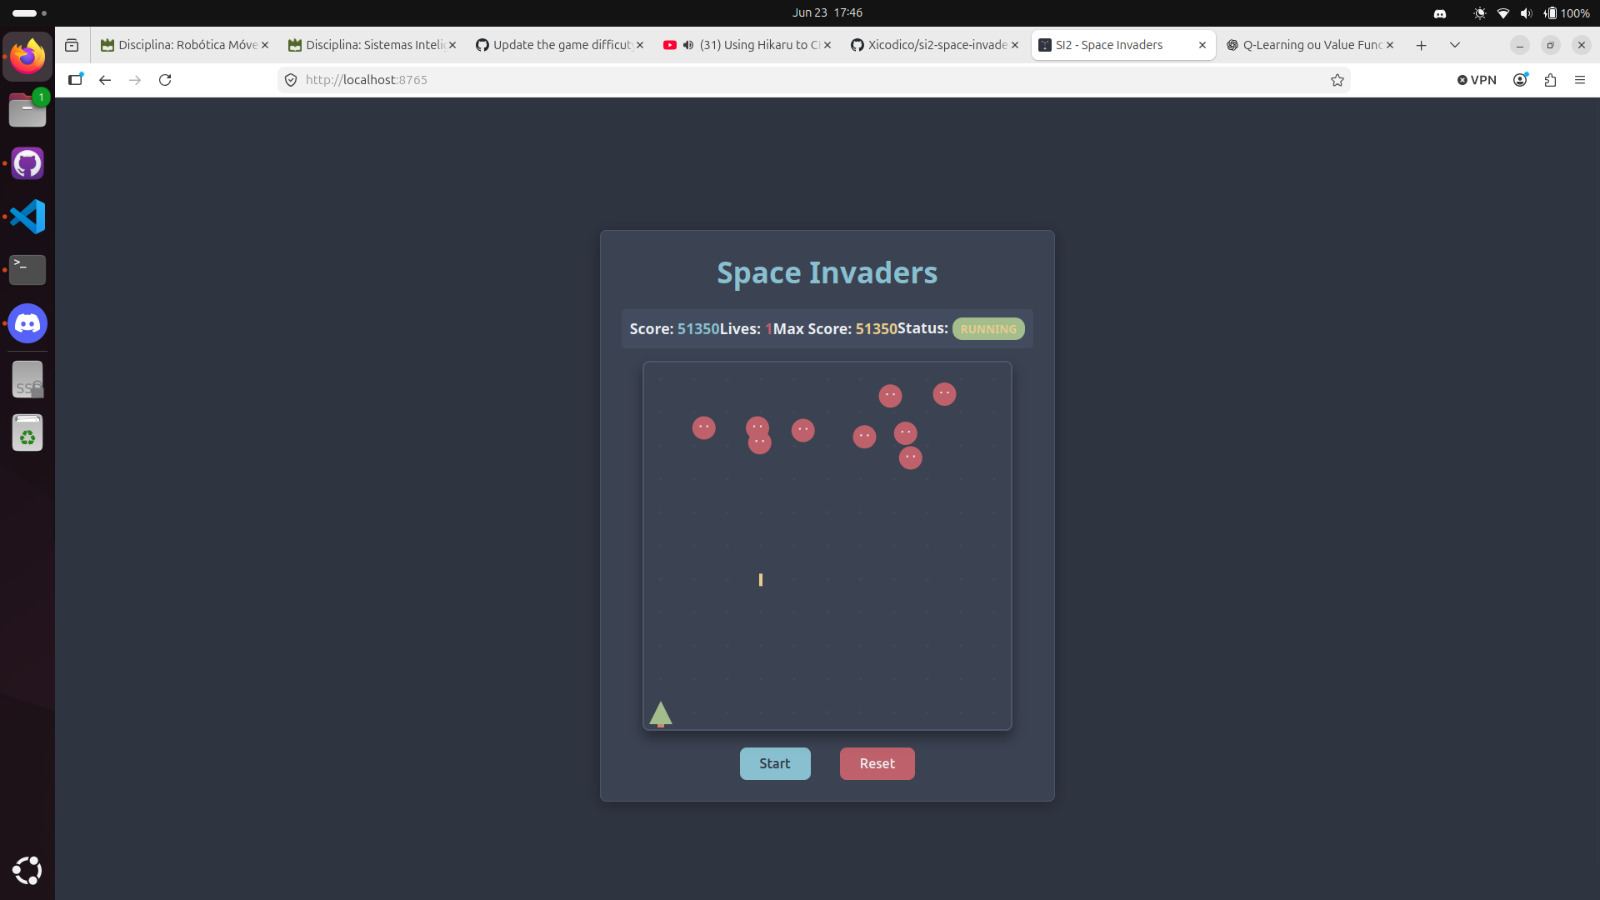
\includegraphics[width=0.9\textwidth]{gameplay.jpg}
    \caption{Exemplo de \textit{gameplay} durante o modo de treino: a nave (triângulo verde)
    posiciona-se sob os alienígenas enquanto um laser está em voo.}
    \label{fig:gameplay}
\end{figure}

\subsection{Abstração do Estado}

O espaço de estado bruto (posições em vírgula flutuante de 10 alienígenas, lasers, etc.) é demasiado grande para Q-Learning tabular. Por isso, o agente extrai seis variáveis para construir o estado:

\begin{enumerate}
    \item \textbf{\texttt{has\_diving\_alien}} (booleano): indica se existe pelo menos um alienígena em mergulho ativo;
    \item \textbf{\texttt{aligned}} (booleano): indica se o jogador está alinhado horizontalmente com o alienígena alvo ($|dx| \leq 1$);
    \item \textbf{\texttt{target\_dx}} (inteiro $\in [-10, 10]$): diferença horizontal entre o alienígena alvo e o jogador, limitada ao intervalo $[-10, 10]$;
    \item \textbf{\texttt{target\_dy}} (inteiro $\in [0, 10]$): metade da diferença vertical (arredondada) entre o alienígena alvo e o jogador, limitada ao intervalo $[0, 10]$;
    \item \textbf{\texttt{can\_shoot}} (booleano): indica se a ação de disparo está disponível, i.e., se o \textit{cooldown} já expirou;
    \item \textbf{\texttt{danger}} (booleano): indica se o agente está em perigo imediato. É verdadeiro quando existe um alienígena em mergulho ($\texttt{has\_diving\_alien} = \text{True}$), a diferença horizontal é muito reduzida ($|dx| \leq 1$) e o alienígena está próximo verticalmente ($dy \leq 3$). Esta variável combate um comportamento excessivamente defensivo que o agente desenvolvia sem ela.
\end{enumerate}

A seleção do \textit{alienígena alvo} segue a seguinte prioridade: se existir um alienígena em mergulho, esse é imediatamente selecionado como alvo; caso contrário, seleciona-se o alienígena ativo mais próximo horizontalmente do jogador. Esta heurística foca o agente na ameaça mais imediata.

O estado é representado como uma tupla Python:

\begin{lstlisting}[language=Python, caption={Construção do estado abstraído}]
current_state = (has_diving_alien, aligned, target_dx, target_dy,
                 can_shoot, danger)
\end{lstlisting}

As variáveis \texttt{can\_shoot} e \texttt{danger} são obtidas da seguinte forma:

\begin{lstlisting}[language=Python, caption={Obtenção das variáveis \texttt{can\_shoot} e \texttt{danger}}]
can_shoot = (
    {"action": "shoot"} in self.current_state.get("valid_actions", [])
)

danger = (
    has_diving_alien and
    abs(target_dx) <= 1 and
    target_dy <= 3
)
\end{lstlisting}

O número total de estados possíveis é:

\begin{equation}
    2 \times 2 \times 21 \times 11 \times 2 \times 2 = 3\,696
    \label{eq:estados}
\end{equation}

onde os fatores correspondem, respetivamente, a \texttt{has\_diving\_alien}, \texttt{aligned},
\texttt{target\_dx}, \texttt{target\_dy}, \texttt{can\_shoot} e \texttt{danger}.
O espaço de $3\,696$ estados é suficientemente compacto para Q-Learning tabular.

\section{Algoritmo de Aprendizagem: Q-Learning Tabular}
\label{sec:qlearning}

\subsection{Espaço de Ações}

O agente dispõe de quatro ações possíveis:

\begin{table}[H]
    \centering
    \begin{tabular}{@{}cll@{}}
        \toprule
        \textbf{ID} & \textbf{Ação} & \textbf{Descrição} \\
        \midrule
        0 & \texttt{move WEST} & Move a nave um passo para a esquerda \\
        1 & \texttt{move EAST} & Move a nave um passo para a direita \\
        2 & \texttt{shoot}     & Dispara um laser na posição atual \\
        3 & \texttt{None}      & Não faz nada (espera) \\
        \bottomrule
    \end{tabular}
    \caption{Espaço de ações do agente.}
    \label{tab:actions}
\end{table}

As ações disponíveis em cada estado são filtradas de acordo com a lista \texttt{valid\_actions} recebida do servidor, garantindo que o agente nunca tenta ações inválidas (e.g., disparar quando o \textit{cooldown} está ativo). A variável \texttt{can\_shoot} é extraída precisamente desta lista para enriquecer a representação de estado.

\subsection{Estrutura da Q-Table}

A Q-table é implementada como um dicionário Python cujas chaves são tuplas de estado e cujos valores são arrays NumPy de dimensão 4 (uma entrada por ação). As entradas são inicializadas a zero por omissão:

\begin{lstlisting}[language=Python, caption={Inicialização preguiçosa da Q-table}]
def get_q_values(self, state):
    if state not in self.q_table:
        self.q_table[state] = np.zeros(len(ACTIONS), dtype=np.float64)
    return self.q_table[state]
\end{lstlisting}

\subsection{Atualização da Q-Table}

A atualização segue a equação clássica do Q-Learning:

\begin{equation}
    Q(s, a) \leftarrow (1 - \alpha)\,Q(s, a) + \alpha\left[r + \gamma \max_{a'} Q(s', a')\right]
    \label{eq:qlearning}
\end{equation}

onde $\alpha$ é a taxa de aprendizagem (\texttt{learning\_rate}), $\gamma$ é o fator de desconto (\texttt{discount\_factor}), $r$ é a recompensa imediata, $s'$ é o próximo estado e $a'$ é a ação ótima nesse estado. Em caso de episódio terminado (\texttt{game\_over}), a componente de valor futuro é anulada:

\begin{equation}
    Q(s, a) \leftarrow (1 - \alpha)\,Q(s, a) + \alpha\, r
\end{equation}

\subsection{Política $\varepsilon$-Greedy}

A política de exploração segue a estratégia $\varepsilon$-greedy: com probabilidade $\varepsilon$ o agente escolhe uma ação aleatória (entre as válidas), e com probabilidade $1 - \varepsilon$ explora a ação com maior valor estimado na Q-table. O valor de $\varepsilon$ decai geometricamente a cada atualização pelo fator \texttt{epsilon\_decay}:

\begin{equation}
    \varepsilon \leftarrow \varepsilon \times \delta_\varepsilon
    \label{eq:epsilon}
\end{equation}

com $\delta_\varepsilon = 0.9995$, garantindo uma transição gradual de exploração para exploração.

\begin{table}[H]
    \centering
    \begin{tabular}{@{}lll@{}}
        \toprule
        \textbf{Hiperparâmetro} & \textbf{Valor} & \textbf{Descrição} \\
        \midrule
        \texttt{learning\_rate} ($\alpha$) & 0.1 & Taxa de aprendizagem \\
        \texttt{discount\_factor} ($\gamma$) & 0.9 & Fator de desconto para recompensas futuras \\
        \texttt{epsilon} ($\varepsilon_0$) & 1.0 & Taxa de exploração inicial \\
        \texttt{epsilon\_decay} ($\delta_\varepsilon$) & 0.9995 & Fator de decaimento de $\varepsilon$ \\
        \texttt{epsilon\_min} & 0.01 & Valor mínimo de $\varepsilon$ \\
        \bottomrule
    \end{tabular}
    \caption{Hiperparâmetros do algoritmo Q-Learning.}
    \label{tab:hyperparams}
\end{table}

\section{Função de Recompensa}
\label{sec:recompensa}

A função de recompensa foi desenhada para guiar o agente em três dimensões comportamentais: penalizar a morte, incentivar o alinhamento com alvos e refletir o progresso de pontuação real.

\subsection{Componentes da Recompensa}

A recompensa é calculada de forma diferida: em cada passo, o agente avalia a transição
$(s_{t-1}, a_{t-1}) \rightarrow s_t$, ou seja, a recompensa atribuída resulta da comparação
entre o estado anterior e o estado atual, após a ação anterior ter produzido efeito no
ambiente. Esta abordagem é necessária porque só após observar o novo estado é possível
quantificar o resultado da ação tomada (e.g., saber se o alinhamento melhorou, se a
pontuação aumentou, ou se o agente morreu).

\begin{enumerate}
    \item \textbf{Penalidade de morte:} quando o episódio termina com \texttt{game\_over}, é aplicada uma penalidade de $-25$, fortemente desincentivando comportamentos que conduzam à morte.
    
    \item \textbf{Custo de ação:} cada ação tem um custo residual de $-0.01$ (para movimento e disparo) ou $-0.05$ (para não fazer nada), penalizando levemente a inação e incentivando o agente a agir proativamente.
    
    \item \textbf{Recompensa de alinhamento:} a diferença absoluta em $x$ entre o agente e o alienígena alvo é comparada entre estados consecutivos: se o agente reduziu a distância horizontal, recebe $+0.1$; se a aumentou, recebe $-0.1$. Isto orienta o movimento lateral para uma posição de tiro.
    
    \item \textbf{Recompensa de pontuação:} o delta de pontuação entre o estado atual e o anterior ($\Delta\,\text{score}$) é adicionado diretamente à recompensa, alinhando o sinal de aprendizagem com o objetivo explícito do jogo.
\end{enumerate}

A recompensa total numa transição é:

\begin{equation}
    r = r_{\text{morte}} + r_{\text{ação}} + r_{\text{alinhamento}} + \Delta\,\text{score}
    \label{eq:recompensa}
\end{equation}

\subsection{Motivação para as Variáveis \texttt{can\_shoot} e \texttt{danger}}

A introdução da variável \texttt{can\_shoot} revelou um problema com a função de recompensa original: a penalização elevada por morte combinada com o aumento do tempo de recarga levava o agente a adotar um comportamento excessivamente defensivo. Quando um alienígena se aproximava na diagonal, o agente tendia a desviar-se mesmo quando poderia disparar, pois não dispunha de informação sobre a disponibilidade do disparo no estado.

A variável \texttt{danger} resolve este comportamento ao distinguir situações de ameaça real daquelas em que o alienígena ainda está suficientemente distante. Apenas quando \texttt{has\_diving\_alien = True}, $|dx| \leq 1$ e $dy \leq 3$ em simultâneo é que a situação é classificada como perigosa, encorajando o agente a disparar ativamente nos outros casos em vez de recuar preventivamente.

\subsection{Condição de Paragem por Desempenho}

Durante o treino, o agente monitoriza continuamente a pontuação. Quando esta atinge ou ultrapassa $15\,000$ pontos numa sessão, o modelo é guardado automaticamente no final dessa sessão. O utilizador pode então optar por parar o treino ou continuar com novas sessões. Esta condição garante que o agente não continue a treinar além do necessário.

\section{Modos de Operação e Persistência}

O agente suporta dois modos de operação, selecionáveis por argumento de linha de comandos:

\begin{itemize}
    \item \textbf{Modo \texttt{train}:} o agente aprende a partir do zero (ou retoma um ficheiro existente), explorando o ambiente e atualizando a Q-table a cada transição. O treino é realizado manualmente, clicando em \textit{Play} no \textit{frontend} para iniciar cada episódio. No final de cada episódio, o modelo é persistido em disco;
    \item \textbf{Modo \texttt{play}:} o modelo guardado é carregado e o parâmetro $\varepsilon$ é fixado a $0.0$, forçando a política puramente greedy sem qualquer exploração.
\end{itemize}

A persistência é feita via \texttt{pickle} sobre o dicionário \texttt{self.q\_table}, guardado por omissão em \texttt{agent.pkl}:

\begin{lstlisting}[language=Python, caption={Serialização e deserialização da Q-table}]
def save(self, file_path: str) -> None:
    with open(file_path, 'wb') as f:
        pickle.dump(self.q_table, f)

def load(self, file_path: str) -> None:
    with open(file_path, 'rb') as f:
        self.q_table = pickle.load(f)
\end{lstlisting}

\section{Resultados e Avaliação}

\subsection{Comportamento Observado}

Após treino, o agente demonstra um comportamento coerente com os objetivos definidos: move-se lateralmente em direção ao alienígena mais próximo, aguarda o alinhamento horizontal antes de disparar, e reage a alienígenas em mergulho priorizando-os como alvo imediato. Graças à variável \texttt{danger}, o agente distingue ameaças reais de aproximações ainda distantes, disparando ativamente quando não está em perigo imediato em vez de recuar preventivamente. A política aprendida é visivelmente superior à do agente aleatório fornecido, que não exibe qualquer direcionamento de movimento ou disparo.

\begin{figure}[H]
    \centering
    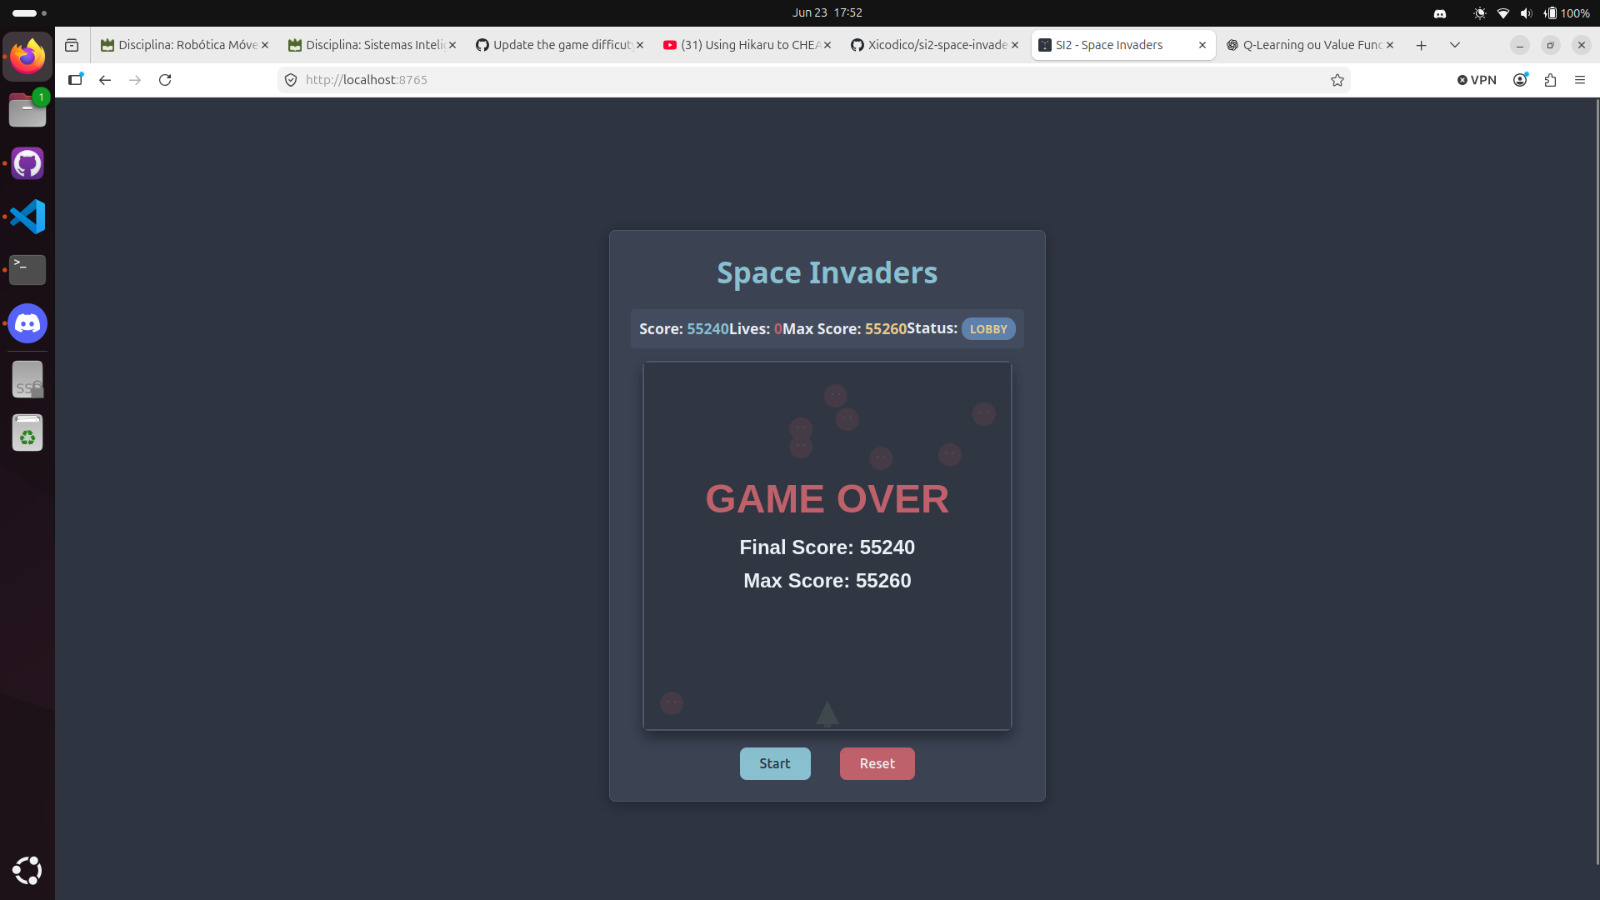
\includegraphics[width=0.9\textwidth]{highscore.jpg}
    \caption{Ecrã de fim de jogo com a pontuação máxima obtida durante o treino (55\,260 pontos, alcançada ao longo de 7 sessões de treino / 21 vidas).}
    \label{fig:highscore}
\end{figure}

\subsection{Limitações}

A principal limitação da abordagem tabular é a incapacidade de generalizar entre estados similares. Estados não visitados durante o treino têm valores Q inicializados a zero, o que pode levar a comportamentos subótimos em configurações de jogo não encontradas anteriormente. 

\section{Utilização de Ferramentas de Apoio}

Recorreu-se a ferramentas baseadas em modelos de linguagem (LLMs), utilizadas exclusivamente para apoio na identificação e correção de pequenos erros de implementação, bem como na formatação de algumas secções do relatório.

\end{document}
